
%(BEGIN_QUESTION)
% Copyright 2007, Tony R. Kuphaldt, released under the Creative Commons Attribution License (v 1.0)
% This means you may do almost anything with this work of mine, so long as you give me proper credit

Determine the proper action for the controller (either {\it direct} or {\it reverse}) to control the process shown in the illustration.  Assume that both the process transmitter and the I/P transducer are direct-acting themselves (greater signal in = greater signal out):

$$\includegraphics[width=15.5cm]{i01753x01.eps}$$

\underbar{file i01753}
%(END_QUESTION)





%(BEGIN_ANSWER)

The controller should be {\bf reverse-acting}.

%(END_ANSWER)





%(BEGIN_NOTES)

{\bf This question is intended for exams only and not worksheets!}.

%(END_NOTES)


